\section{Network Debugger}
\subsection{Overview}

The user of the network debugger provides a model of the network and a
set of experiments. For each experiment, the network debugger assesses
whether the experiment is consistent with the model, explaining why
(with a queryable proof) or why not (with queryable minimal fixes).

\subsection{Demonstration}

For purpose of demonstration, we will use the small network shown in Figure~\ref{figure:network}.
The user code which specifies this network model is shown in Listing~\ref{listing:network-model-def}.

The set of experiments in Listing~\ref{listing:experiments} tests our
model. In order to test our system, we purposefully introduced some
inconsistencies in our model with respect to the experiments:
\begin{itemize}
\item {\small\tt reaction r1} has its reactants and products swapped.
\item {\small\tt reaction r2} has no enzymes catalyzing it.
\item {\small\tt reaction r4} shouldn't actually be part of our model.
\end{itemize}

\begin{figure}[htb]
\centering
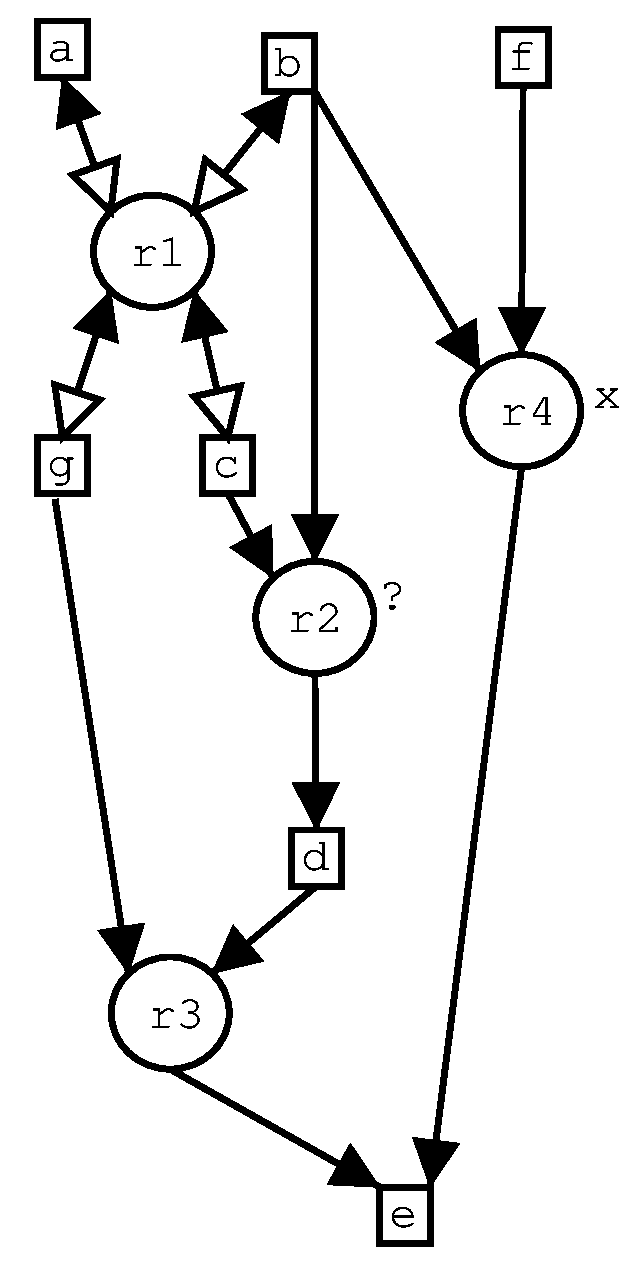
\epsfig{file=demo.eps, height=3in, width=1.5in}
\caption{\label{figure:network} Example Metabolic Network}
\end{figure}

\begin{lstlisting}[label={listing:network-model-def},caption={Network Model}]
(network-debugger demo 
  :debugging t 
  :abducting t 
  :rules :extended-reactions)

(reaction r1 
  :reactants (c g) 
  :products (a b) 
  :enzymes (e1))

(reaction r2 
  :reactants (b c) 
  :products (d))

(reaction r3 
  :reactants (d g) 
  :products (e) 
  :enzymes (e3))

(reaction r4 
  :reactants (b f) 
  :products (e) 
  :enzymes (e4))

(enzyme e1 g1)
(enzyme e3 g3 g3p)
(enzyme e4 g4)
\end{lstlisting}

\begin{lstlisting}[label={listing:experiments},caption={Experiments}]
(experiment 
 positive 
 (a b d) 
 :growth? t 
 :essential-compounds (a e))

(experiment 
 negative 
 (a) 
 :growth? nil 
 :essential-compounds (a e))

(experiment 
 false-positive 
 (a b f) 
 :growth? nil 
 :essential-compounds (a e) 
 :knock-outs (g1))

(experiment
 false-negative
 (a b)
 :growth? t
 :essential-compounds (a e))
\end{lstlisting}

We immediately get the following feedback when loading the set of
experiments:
\begin{itemize}
\item Experiments {\small\tt positive} and {\small\tt negative} are consistent with the model.
\item Experiment {\small\tt false-positive} is not consistent with the model. Needs:
\begin{itemize}
\item {\small\tt ( (NOT (GENE-ON G4)) )}
\end{itemize}
\item Experiment {\small\tt false-negative} is not consistent with the model. Needs:
\begin{itemize}
\item {\small\tt ( (NUTRIENT E) )}
\item {\small\tt ( (NUTRIENT D) )}
\item {\small\tt ( (REACTION-ENABLED R2) )}
\item {\small\tt ( (NUTRIENT F) )}
\end{itemize}
\end{itemize}

Notice that the network debugger suggested enabling {\small\tt
reaction r2} and disabling {\small\tt reaction r4} to fix our model.

Once an experiment is consistent with the model, the network debugger
can explain why by providing a proof and allowing the user to query
this proof. For example, after loading the experiment {\small\tt
positive}, the user can type {\small\tt (explain
'experiment-consistent)} to get a Suppes-style proof. The user can
query the facts that play a role in the proof using {\small\tt
all-antecedents}. For example, {\small\tt (all-antecedents
'experiment-consistent '((reaction-enabled ?r) (reaction-reversible
?r)))} returns {\small\tt ((REACTION-ENABLED R3) (REACTION-ENABLED R1)
(REACTION-REVERSIBLE R1))}. As a shortcut, it is possible to list
reactions that had to explicitly be assumed reversible for the proof:
{\small\tt (explicit-reversibility)} returns {\small\tt
(R1)}. Similarly, {\small\tt (explicit-gene-expression)} returns which
genes had to explicitly be assumed on for the proof.

\subsection{Specification}
\subsection{Implementation}
